\documentclass[12pt]{article}
\usepackage{latexsym}
\usepackage{epsfig}
\usepackage{amsmath}
\usepackage[edges]{forest}


\setlength{\topmargin}{0in}
\setlength{\leftmargin}{0in}
\setlength{\textwidth}{6in}
\setlength{\textheight}{9.5in}
\setlength{\parindent}{0.2in}
\setlength{\parskip}{.08in}
\voffset = -.45in
\hoffset = -.5in
\def\filledbox{\vrule height 1.8ex width .8ex depth -.1ex } % square bullet
\newcommand{\qed}{\large ~$\Box$ \normalsize}
%
%\newtheorem{thm}{Theorem}
%\newenvironment{theorem}{\begin{thm}\ \rm}{\end{thm}}
%
%\newtheorem{lem}{Lemma}
%\newenvironment{lemma}{\begin{lem}\ \rm}{\end{lem}}
%
\newtheorem{theorem}{Theorem}
\newtheorem{lemma}{Lemma}
\newtheorem{corollary}{Corollary}
\newenvironment{proof}{{\noindent \bf Proof\ \ }}{\qed}
\newenvironment{proofsketch}{{\noindent {\bf Proof}\ (sketch)\ \ }}{\qed}
%
\def\shh{\skew3\hat{\hat s}}
\def\dhh{\skew6\hat{\hat d}}
\begin{document}
\newcommand{\I}{\mbox{{\em Int}}}
\newcommand{\lt}{\mbox{{\em left}}}
\newcommand{\rt}{\mbox{{\em right}}}
\newcommand{\ld}{\Delta^l}
\newcommand{\rd}{\Delta^r}
\newcommand{\lsp}[1]{\large\renewcommand{\baselinestretch}{#1}\normalsize}
\newcommand{\hsp}{\hspace{.2in}}

\def\Endwhile{\mbox{\bf endwhile\ }}
\def\Or{\mbox{\bf or\ }}
\def\Do{\mbox{\bf do\ }}
\def\Downto{\mbox{\bf downto\ }}
\def\Int{\mbox{\bf int\ }}
\def\To{\mbox{\bf to\ }}
\def\Repeat{\mbox{\bf repeat\ }}
\def\Until{\mbox{\bf until\ }}
\def\Return{\mbox{\bf return\ }}
\def\Not{\mbox{\bf not\ }}
\def\And{\mbox{\bf and\ }}
\def\For{\mbox{\bf for\ }}
\def\Foreach{\mbox{\bf foreach\ }}
\def\Else{\mbox{\bf else\ }}
\def\Elseif{\mbox{\bf elseif\ }}
\def\End{\mbox{\bf end\ }}
\def\If{\mbox{\bf if\ }}
\def\Mod{\mbox{\bf \ mod\ }}
\def\Then{\mbox{\bf then\ }}
\def\While{\mbox{\bf while\ }}
\def\Output{\mbox{\bf output\ }}


\lsp{1}
\pagestyle{plain}
\hfill Ally Smith
\begin{center}
{\bf
% Worksheet title here %
Maze Project
}
\end{center}

\section{Modelling}

I modeled the maze using two separate graphs, one for forwards traversal and
one for backwards. Each time the search lands on a circled node, it switches to
the other graph, emulating the rules of Apollo's maze with Diana. Additionally,
each node connects to the opposite color of nodes within the path of its
direction. For example, a blue node facing northeast would connect to any red
nodes along the NE diagonal from the original node in the forwards graph. In
the backwards graph, the connections would be made with red nodes in the SW
direction. Below is a small maze + the corresponding graphs:

\begin{center}
    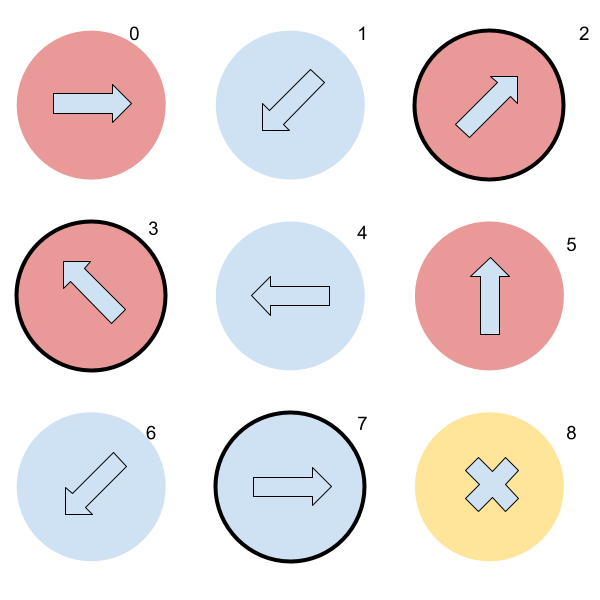
\includegraphics[width=5in]{examplemaze.png}

    \textbf{Figure 1:} Example maze with a few circled nodes,\\
    each labeled with their index.

    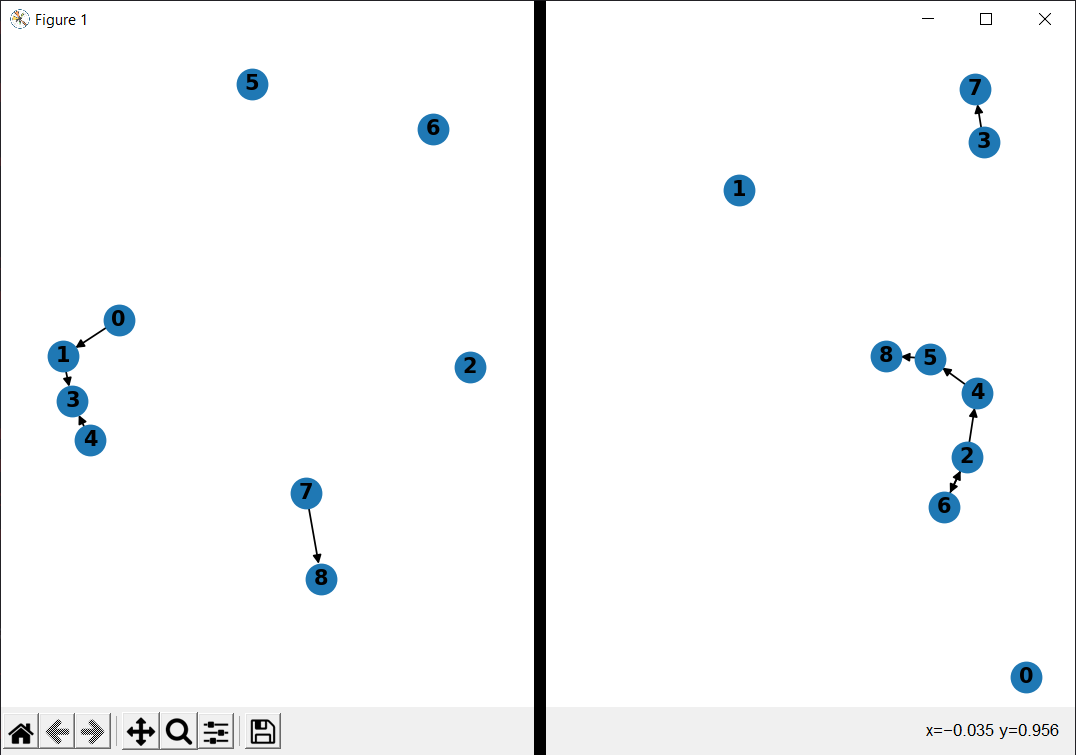
\includegraphics[width=4in]{graphs.png}

    \textbf{Figure 2:} The graphs, recreated manually. The forward
    edges are on the top portion, and the backwards on the bottom.
    Lines that cross from top to bottom land on a circle and therefore
    must switch which part of the graph it is in.
\end{center}
\pagebreak

Using this model for the problem, we can apply a breadth-first search algorithm
to find the shortest path through the maze. We can convince ourselves this is
the case by imagining this as one large graph rather than two graphs, as they are
not disjoint. We simply draw lines from the circled nodes to the corresponding nodes
in the opposite direction graph. This allows us to merge the two together into a 
single graph, and therefore BFS will always find a path through the maze if one exists.

\section{Code}
Below is the code that I used to work on this project, including the BFS
algorithm I used to find the path through Apollo's maze. At the end of the
pictures, you will see the output of my program
\begin{center}
    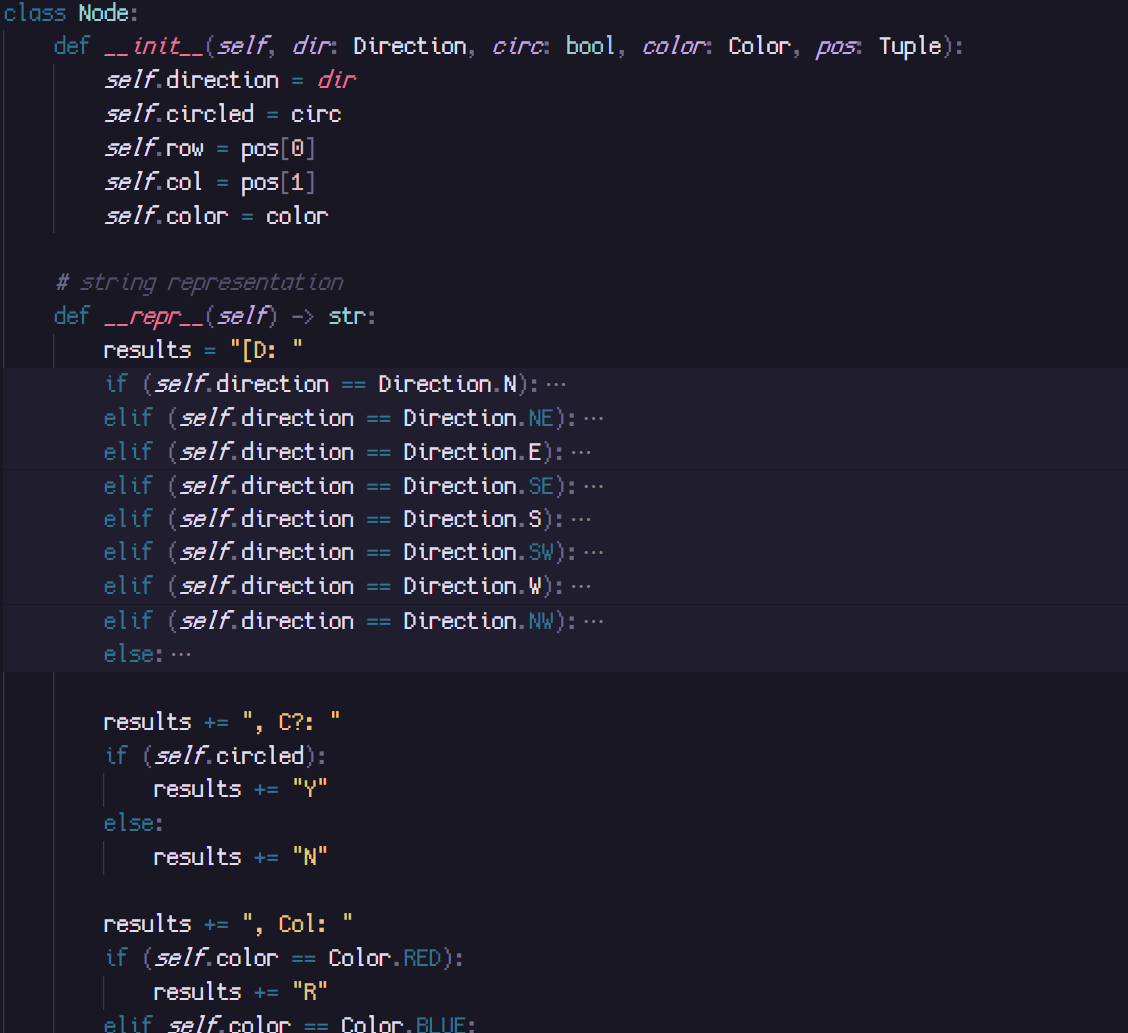
\includegraphics[width=5in]{node.png}

    \textbf{Figure 3:} The basic node class I used to store the arrow \& circle
    information.

    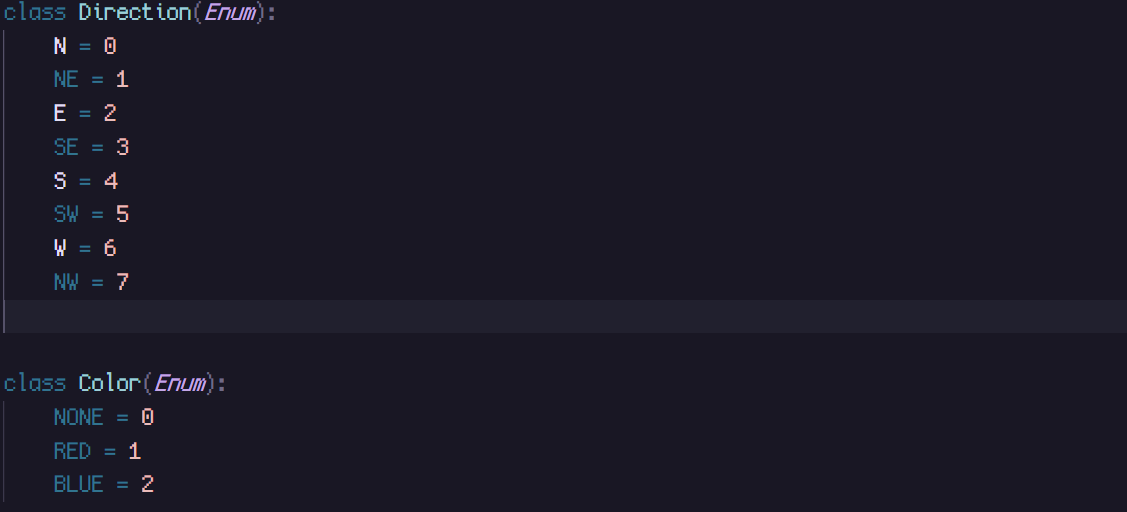
\includegraphics[width=5in]{properties.png}

    \textbf{Figure 4:} Basic enumerations I used to store data in a more
    readable fashion.

    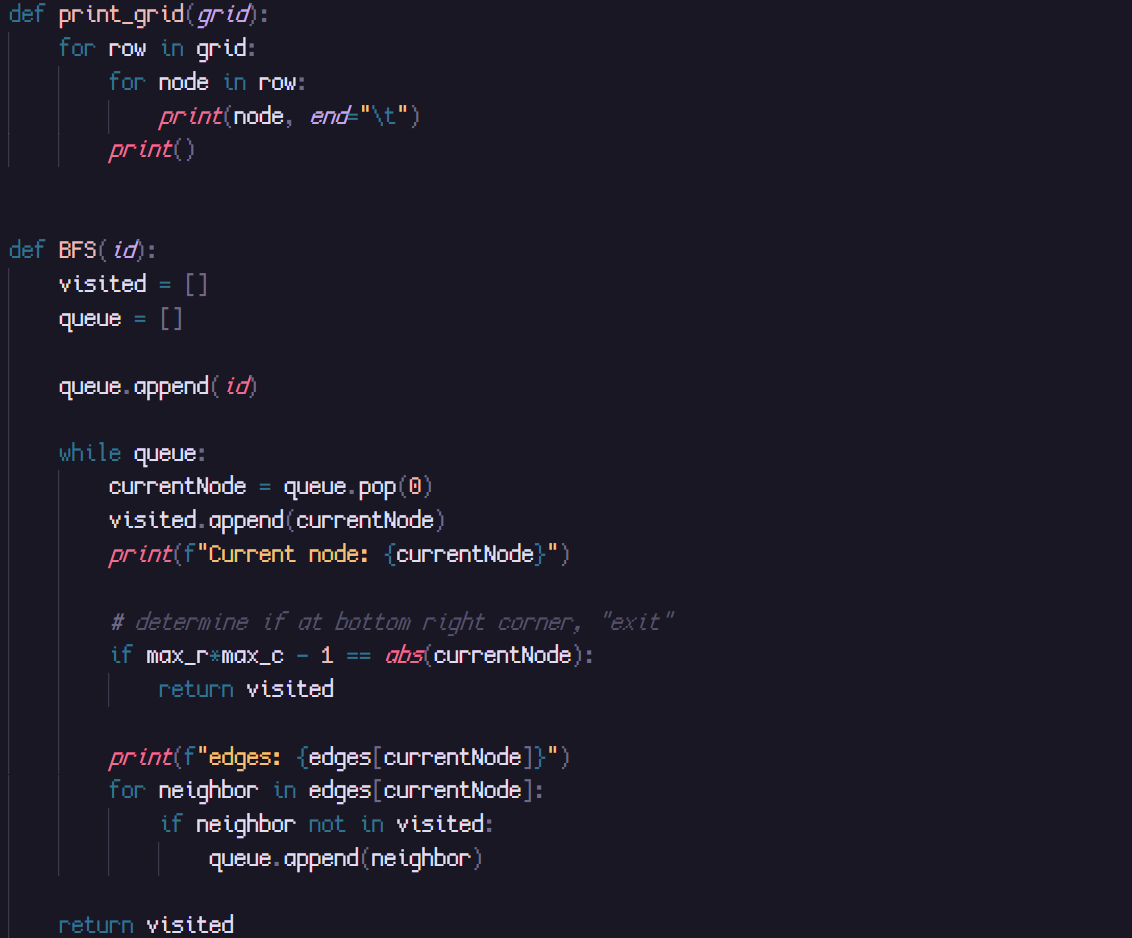
\includegraphics[width=5in]{algorithm.png}

    \textbf{Figure 5:} Here is the BFS algorithm that I implemented.

    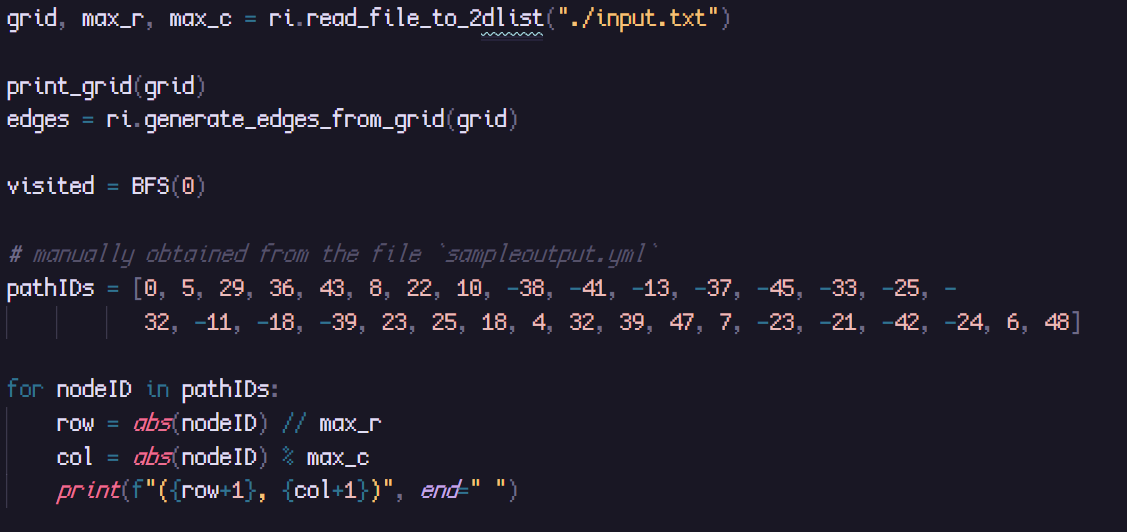
\includegraphics[width=5in]{driver.png}
    
    \textbf{Figure 6:} This is the code I used to drive my program, plus
    the code I used to calculate the coordinates in the appropriate output
    format for the assignment from the node IDs that I was using.

    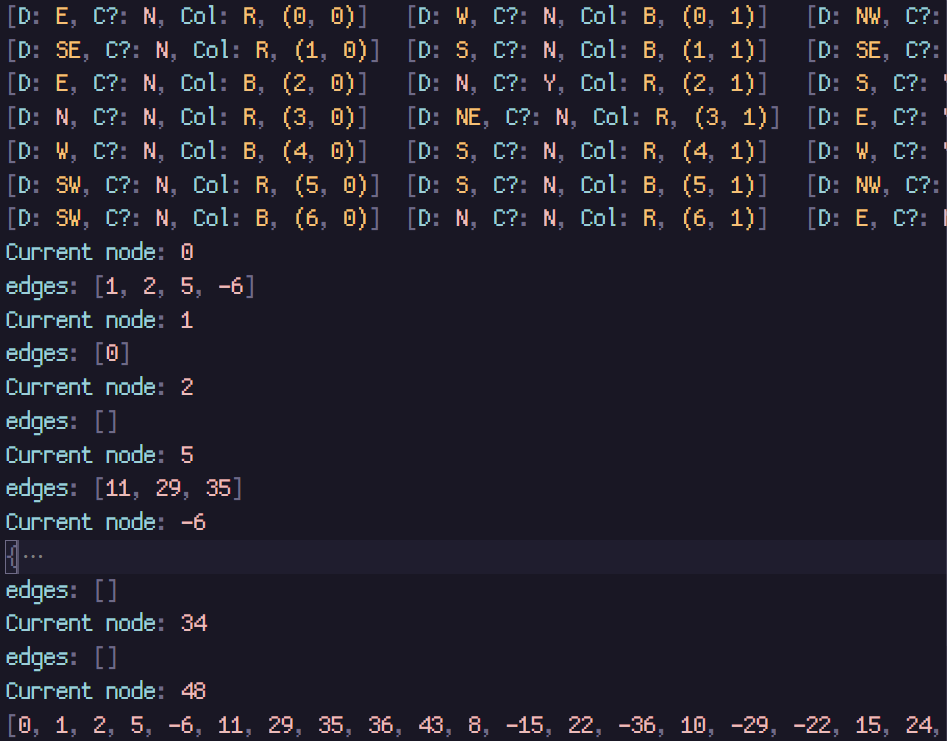
\includegraphics[width=5in]{sample-output.png}

    \textbf{Figure 7:} Above is the sample output of the program. It prints
    the grid, then prints each node as it gets to it and its neighbors. By 
    working from the bottom up, you can find which node led you to where you
    are, and if you work all the way to the top you can determine the entire
    route. I identified my nodes starting at 0 up to $(r\times c) - 1$, as well
    as negative values for the backwards counterpart to each node, which can be
    seen at the bottom, which is the list of nodes in the order they were visited.
\end{center}
\pagebreak

\section{Results}
When converted to the proper format, this is the output that I got:

(1, 1) (1, 6) (5, 2) (6, 2) (7, 2) (2, 2) (4, 2) (2, 4) (6, 4) (6, 7) (2, 7)\\
(6, 3) (7, 4) (5, 6) (4, 5) (5, 5) (2, 5) (3, 5) (6, 5) (4, 3) (4, 5) (3, 5)\\
(1, 5) (5, 5) (6, 5) (7, 6) (2, 1) (4, 3) (4, 1) (7, 1) (4, 4) (1, 7) (7, 7)

\end{document} 
